\documentclass[11pt]{article}
\usepackage[a4paper, hmargin={2.8cm, 2.8cm}, vmargin={2.5cm, 2.5cm}]{geometry}
\usepackage[table, dvipsnames]{xcolor} \usepackage{eso-pic}
\usepackage{graphicx}
\usepackage{placeins}
\usepackage{amsmath}
\usepackage{mwe}
\usepackage[utf8]{inputenc}
\usepackage[T1]{fontenc}
\usepackage{verbatim}
\usepackage[all]{xy}
\usepackage{multirow}
\usepackage{amssymb}
\usepackage{svg}
\usepackage{neuralnetwork}
\usepackage{listings}
\usepackage{glossaries}
\usepackage{adjustbox}
\usepackage{hyperref}
\usepackage{multicol}
\usepackage{color}
\usepackage{url}
\usepackage{tabu}
\usepackage{tcolorbox}
\usepackage{enumerate}
\usepackage{caption}
\usepackage{mwe}
\usepackage{subfig}
\usepackage{float}
\usepackage{pdflscape}
\usepackage{pdfpages}
\usepackage{amsthm}
\usepackage{sverb}
\usepackage[linesnumbered,ruled,vlined]{algorithm2e}
\usepackage{paralist}
\usepackage{array}
\usepackage{bbm}
\usepackage[normalem]{ulem}
\usepackage[square]{natbib}

\author{
    \begin{tabular}{ccc}
    \Large{August V. S\o rensen} & \& & \Large{Magnus N. Stavngaard} \\
    august.vinkel@gmail.com      &    & magnus@stavngaard.dk         \\
    NCB360                       &    & MZC887
    \end{tabular}
}

\title{
    \vspace{3cm}
    \Huge{Authorship Verification} \\
    \Large{Deep Learning Based Methods for Authorship Verification}
}

\usepackage{fancyhdr}
\pagestyle{fancy}

\lhead{University of Copenhagen}
\rhead{August V. S\o rensen \& Magnus N. Stavngaard}
%\cfoot{}
%\rfoot{\thepage}

\begin{document}

    \AddToShipoutPicture*{\put(0,0){\includegraphics*[viewport=0 0 700 600]{pictures/report/ku-farve}}}
    \AddToShipoutPicture*{\put(0,602){\includegraphics*[viewport=0 600 700 1600]{pictures/report/ku-farve}}}
    \AddToShipoutPicture*{\put(0,0){\includegraphics*{pictures/report/ku-en}}}
    \clearpage\maketitle
    \thispagestyle{empty}
    \newpage

    \pagenumbering{roman}
    \setcounter{page}{1}

    \section{Introduction}

    During the last 6 months we have created a system designed to determine if a
    secondary school student possibly made use of a ghostwriter. Throughout this
    description we will call this process authorship Verification . This system
    is intended be a tool that assists teacher in more accurately determining
    the authenticity of an assignment, while also providing a description of
    what factors contributed to the decision the system made.

    The goal we set out to meet was keeping the amount of false accusation under
    10\%, while catching 95\% of the students who made use of a ghostwriter.
    Keeping a low amount of false accusation was the primary goal of the two,
    meaning that it would be acceptable if sacrificed the amount of students we
    caught if resulted in a low amount of false accusations.

    The system we created was intended to be supplementary, by aiding teachers
    in their decision, not making it for them.

    This summary will go through the major points of our master thesis.
    If any more information is desired, please refer to the full thesis.


    \section{Data}

    The data used for the creation of this system was provided by MaCom. We made
    use a set consisting of 10.000 authors, spread across several different
    schools.

     
    \section{The System}

    The system we produced consists of two parts. A neural network
    and a prediction system.

    The way the our system works is when a student hands in an assignment,
    the assignment ($t$) and the student ID ($\alpha$) is given to our system.
    The assignment $t$ is then compared to each of the assignment previously
    created by $\alpha$, each producing a score indicating how alike the two
    assignments are.

    It then takes a weighted average over these likeness scores. The weight
    of assignment is based on the time the assignment was submitted in months
    relative to the assignment $t$, and how long each text is, as smaller text
    are less indicative of a students' writing style. A simple model of the proces
    can be seen in Figure \ref{fig:model}.

    \begin{figure}
    \centering
    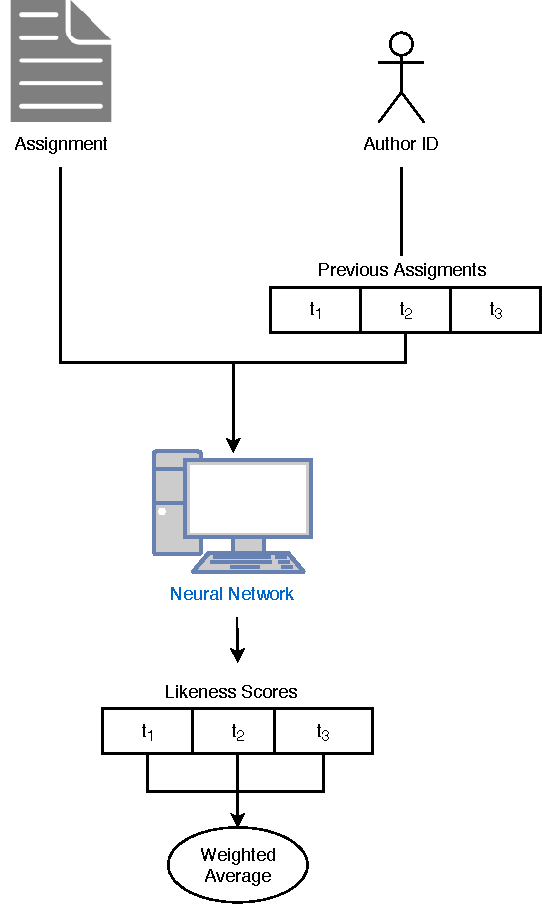
\includegraphics[width=0.5\textwidth]{./pictures/Model}
    \caption{A simply illustration of the likeness computation performed
            when our system receives a text for analysis}
    \label{fig:model}
    \end{figure}


    In other words previous assignments that were submitted at a point
    in time near $t$ will be weighed higher. Additionally texts
    that are longer will also be rated higher.

    This weighing scheme was decided after performing a multiplicity of
    experimenting with different weighing functions, using a subset of the
    10.000 authors we were provided.

    If this weighted average likeness exceeds a certain threshold, the
    assignment is considered non-ghostwritten. This threshold
    is what we use to control the accusation error of our system,
    as it allows us to control how certain our system has to be in
    its' decision making

    \section{Teacher Feedback}

    What the system looks for is the usage of certain combinations of
    characters. After our neural network has learned by looking a many thousands
    of student assignments, it has learned how the typical student writes.
    It is using this, that when the system decides a student isn't the author
    of a text, it will be able to provide evidence to back up its claims.

    % TODO: How to explain this? :O 
    

\end{document}
